%Beamer class
\documentclass{beamer}

\usepackage[czech]{babel}
\usepackage[utf8]{inputenc}
\usepackage{fontenc}
\usepackage{tgheros}
\usepackage{array}
\usepackage{color}
\usepackage{hyperref}
\usepackage{fancyvrb} % pro verbatim

\usetheme{AnnArbor}
\usecolortheme{crane}


\title[KiCAD Eeschema]{Tvorba schéma zapojení v KiCAD}
\subtitle[KEO] {Konstrukce a realizace elektronických obvodů}
\author[Brejcha]{\texorpdfstring{Michal Brejcha\newline\url{brejcmic@fel.cvut.cz}}{Michal Brejcha}}
\institute[ČVUT]{ČVUT v Praze, FEL}
\date[Praha, 2021]{Praha, 2021}

%------------------------------------------------------------------------------
%Konstanty a definice
%------------------------------------------------------------------------------
\newtheorem{myDef}{}
\newcommand{\kicadVersion}{5.1.10.}

\begin{document}
%------------------------------------------------------------------------------
%Uvodni slajd
%------------------------------------------------------------------------------
\frame{\titlepage}

\begin{frame}
\frametitle{Obsah} 
\tableofcontents
\end{frame}

\AtBeginSection[]
{
  \begin{frame}
    \frametitle{Téma}
    \tableofcontents[currentsection]
  \end{frame}
}

%------------------------------------------------------------------------------
% Založení projektu
%------------------------------------------------------------------------------
\section{\texorpdfstring{Založení projektu}{Zalozeni projektu}}
\subsection{\texorpdfstring{Příprava nového projektu}{Priprava noveho projektu}}
%------------------------------------------------------------------------------
\begin{frame}
	\frametitle{Nový projekt}
	\begin{columns}
	
		\column{.5\textwidth}
		\begin{center}
			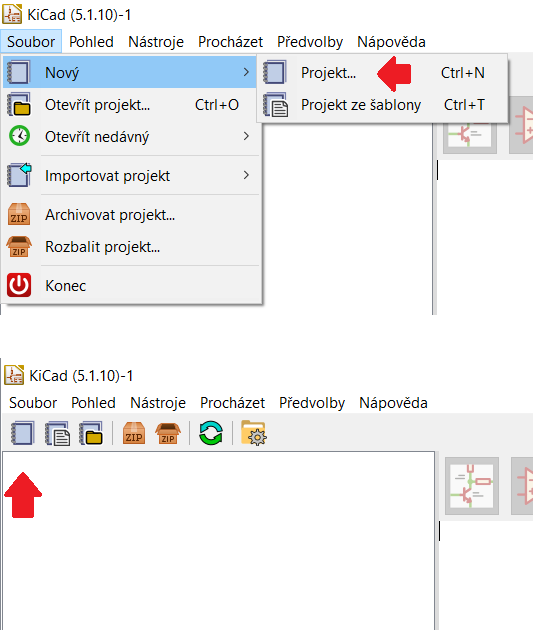
\includegraphics[width=\textwidth]{obr/prj_novy01.png}
		\end{center}
	
		\column{.5\textwidth}
		\textbf{Možnosti:}
		\begin{itemize}
			\item $\downarrow$ Soubor $\downarrow$ Nový $\downarrow$ Projekt
			\item CTRL+N
			\item Modrá ikona notýsku úplně vlevo
		\end{itemize}
	\end{columns}
\end{frame}
%------------------------------------------------------------------------------
\begin{frame}
	\frametitle{Nový projekt}

		\begin{center}
			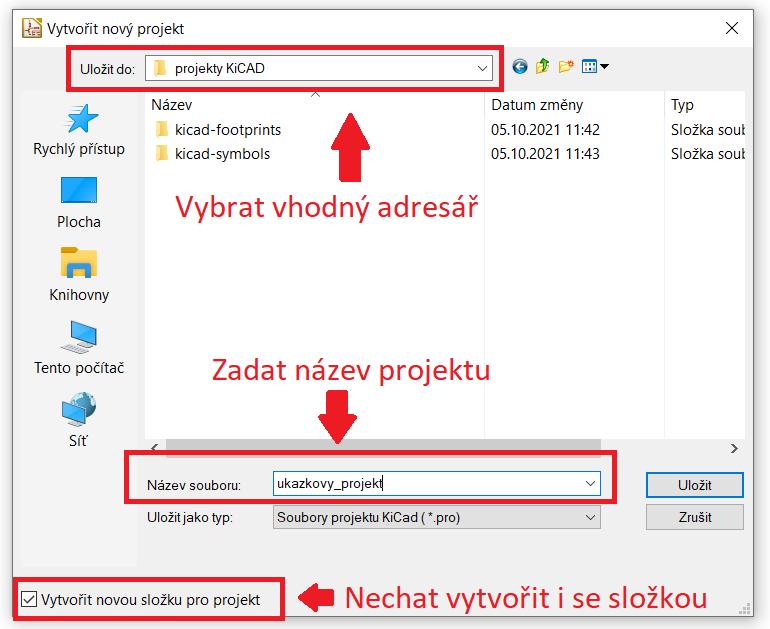
\includegraphics[width=0.7\textwidth]{obr/prj_novy02.png}
		\end{center}
    
\end{frame}
%------------------------------------------------------------------------------
\begin{frame}
	\frametitle{Aktivní projekt}

		\begin{center}
			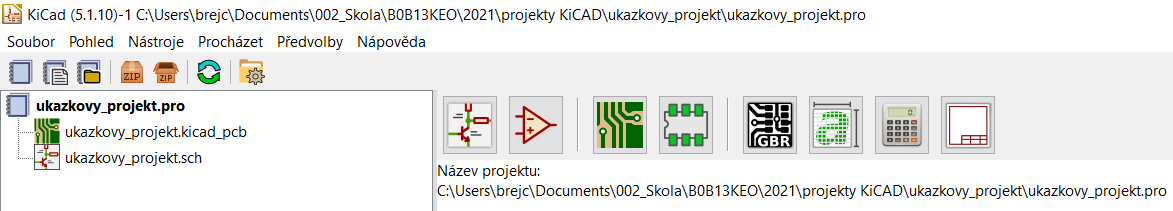
\includegraphics[width=\textwidth]{obr/prj_novy03.png}
		\end{center}
    
		
		\begin{itemize}
			\item Vlevo se je souborová struktura projektu,
			\item ikony pro jednotlivé programy (Návrh schématu, Editor součástek, atd.) jsou aktivní a programy automaticky pracují s projektovými soubory.
		\end{itemize}
		
\end{frame}
%------------------------------------------------------------------------------


%------------------------------------------------------------------------------
\subsection{\texorpdfstring{Přidání vlastních knihoven}{Pridani vlastnich knihoven}}
%------------------------------------------------------------------------------
\begin{frame}
	\frametitle{Zadání cest k vlastním knihovnám}
	\begin{columns}
	
		\small
		\column{.45\textwidth}
		\textbf{Dva typy knihoven:}
		\begin{itemize}
			\item schématické značky a
			\item pouzdra.
		\end{itemize}
		
		\textbf{Editace cest:}
		\begin{enumerate}
			\item přímo z projektového menu,
			\item pro schématické značky z programu \uv{Editor schémat},
			\item pro pouzdra z programu \uv{Návrh DPS},
		\end{enumerate}
		
		\textbf{Vždy pomocí:}
		
		$\downarrow$ Předvolby $\downarrow$ Správa knihoven $[$součástek $|$ pouzder$]$
	
		\column{.55\textwidth}
		\begin{center}
			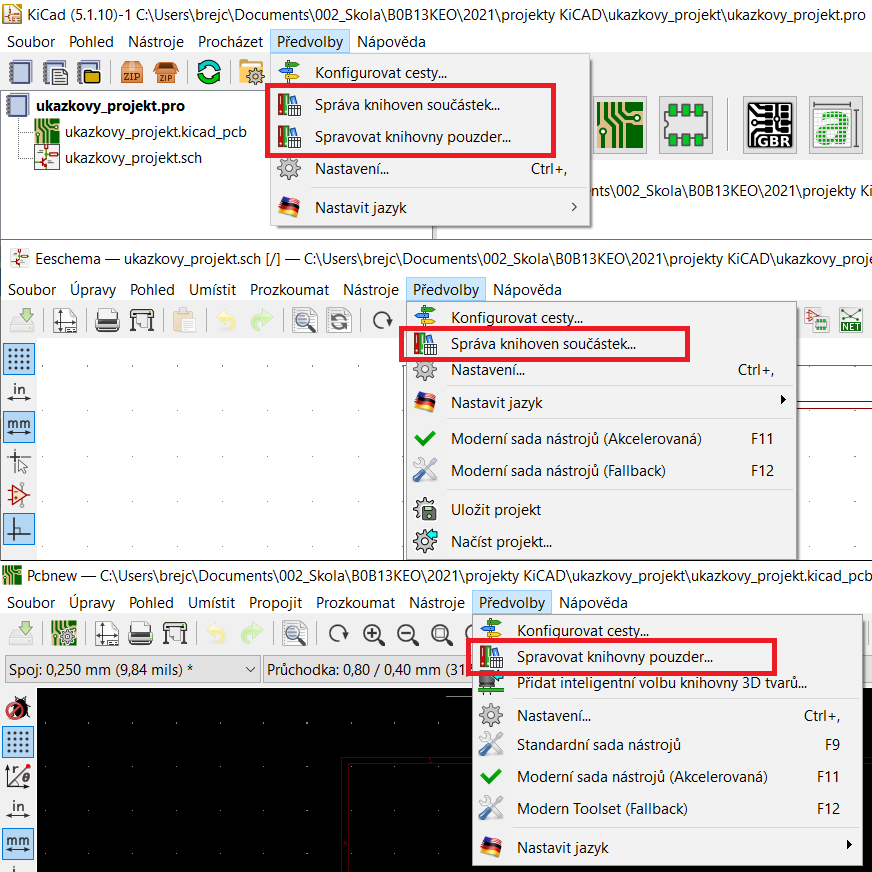
\includegraphics[width=\textwidth]{obr/knihovny01.png}
		\end{center}
	
	\end{columns}
\end{frame}
%------------------------------------------------------------------------------
\begin{frame}
	\frametitle{Zadání cest k vlastním knihovnám}
	
	\textbf{Cesty ke knihovnám jsou:}
	\begin{itemize}
		\item \uv{Globální}, pak platí pro jakýkoliv projekt na daném PC,
		\item \uv{Specifické pro projekt}, pak se týkají jen konkrétního projektu.
	\end{itemize}
	
	\vspace{0.3cm}
	V rámci předmětu B0B13KEO nebudeme nahrazovat cesty ke globálním knihovnám. Pouze je deaktivujeme a jako aktivní označíme přidané projektové knihovny.
	
	\vspace{0.3cm}
	Cesty ke knihovnám se ukládají a dají měnit editováním textových souborů:
	
	\begin{itemize}
		\item sym-lib-table
		\item fp-lib-table
	\end{itemize}
		
\end{frame}
%------------------------------------------------------------------------------
\begin{frame}
	\frametitle{Zadání cest ke knihovnám - schematické značky}

		\begin{center}
			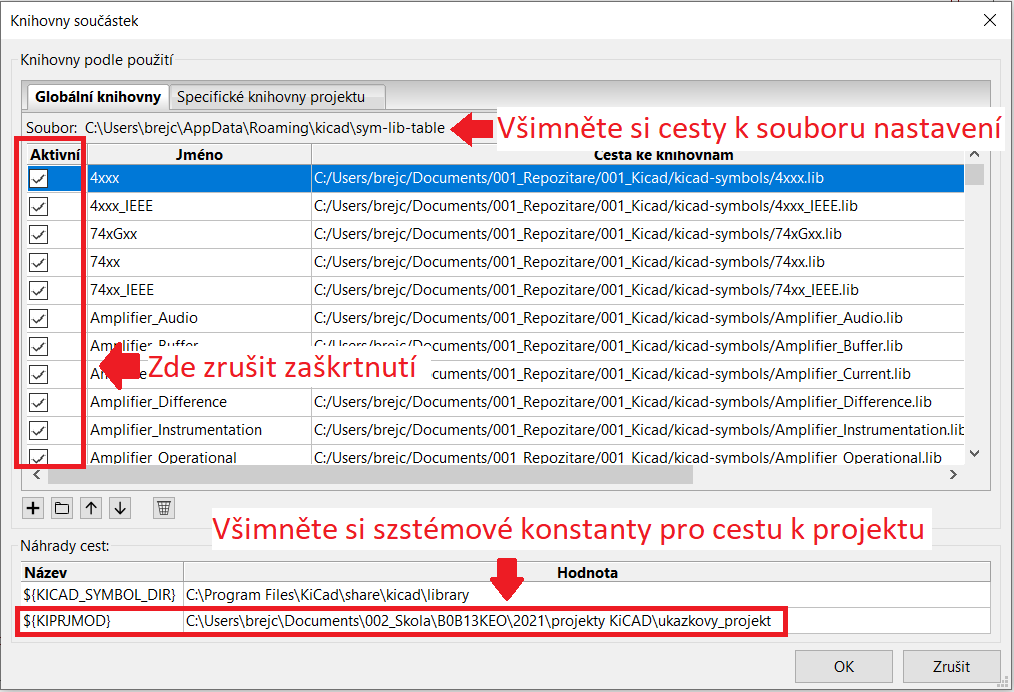
\includegraphics[width=0.85\textwidth]{obr/knihovny02.png}
		\end{center}
		
\end{frame}
%------------------------------------------------------------------------------
\begin{frame}
	\frametitle{Zadání cest ke knihovnám - schematické značky}

		\begin{center}
			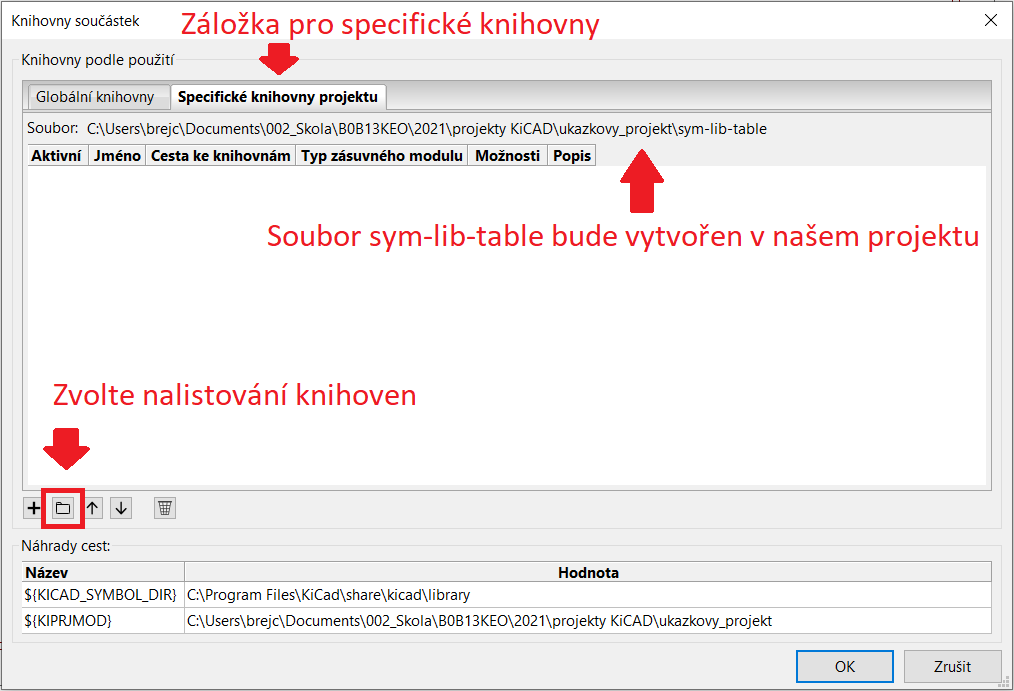
\includegraphics[width=0.85\textwidth]{obr/knihovny03.png}
		\end{center}
		
\end{frame}
%------------------------------------------------------------------------------
\begin{frame}
	\frametitle{Zadání cest ke knihovnám - schematické značky}

		\begin{center}
			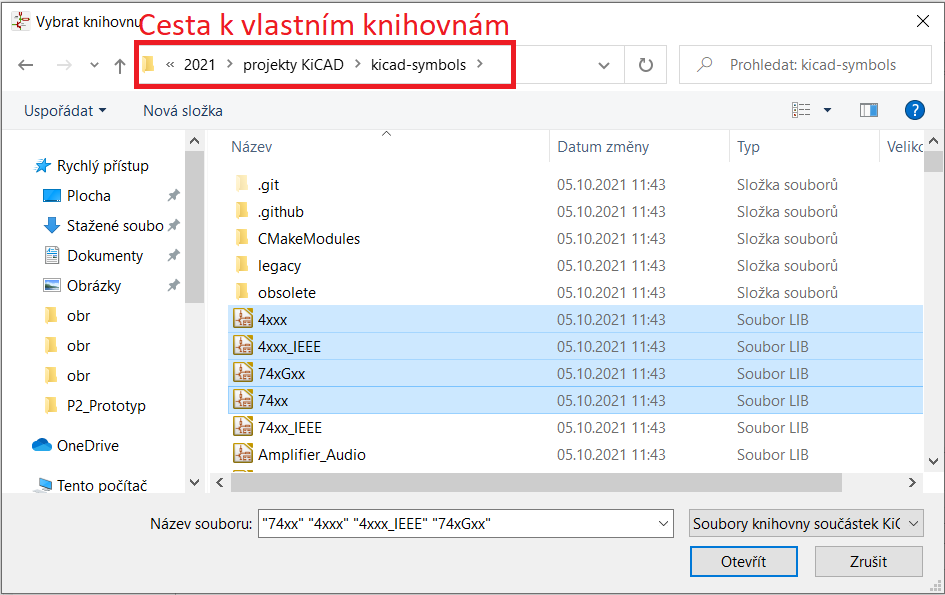
\includegraphics[width=0.7\textwidth]{obr/knihovny04.png}
		\end{center}
	  
		\begin{itemize}
			\item Nastavte cetu k vlastním knohovnám
			\item a pomocí klávesy shift nebo ctrl vyberte všechny soubory *.lib
		\end{itemize}
\end{frame}
%------------------------------------------------------------------------------
\begin{frame}
	\frametitle{Zadání cest ke knihovnám - schematické značky}

		\begin{center}
			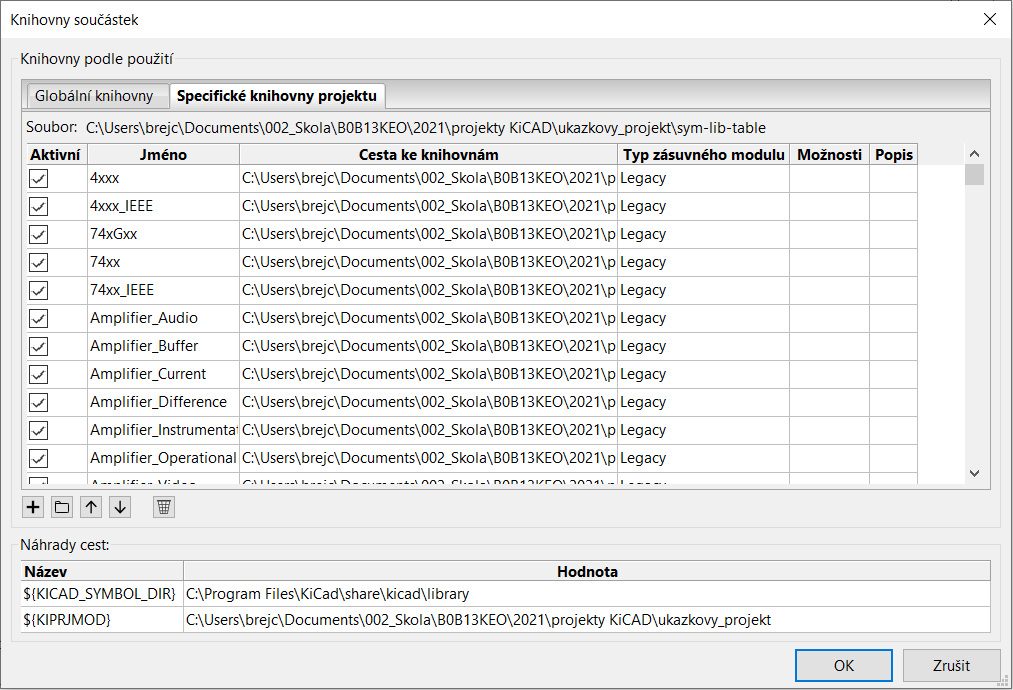
\includegraphics[width=0.85\textwidth]{obr/knihovny05.png}
		\end{center}
		
\end{frame}
%------------------------------------------------------------------------------
\begin{frame}[fragile]
	\frametitle{Zadání cest k vlastním knihovnám}
	\small
	Všimněte si, že všechny soubory jsou zadány absolutní cestou. To může být nevýhodné, pokud s někým sdílíte projekt nebo zálohujete tento projekt na jiném počítači (GIT apod.).
	
	\vspace{3mm}
	Nejvhodnější způsob je zadání relativních cest pomocí systémové proměnné \$$\{$KIPRJMOD$\}$, která ukazuje na adresář našeho projektu.
	
	\vspace{3mm}
	Jelikož vkládané knihovny jsou v našem případě ve stejné složce jako projekty, je nutné přepsat začátek všech cest:
	
	\begin{verbatim*}
		C:\Users\brejc\Documents\002_Skola\B0B13KEO\2021\projekty_KiCAD\
	\end{verbatim*}
	
	na tvar:
	
	\$\verb+{KIPRJMOD}/../+
		
\end{frame}
%------------------------------------------------------------------------------
\begin{frame}
	\frametitle{Zadání cest ke knihovnám - schematické značky}

		\begin{center}
			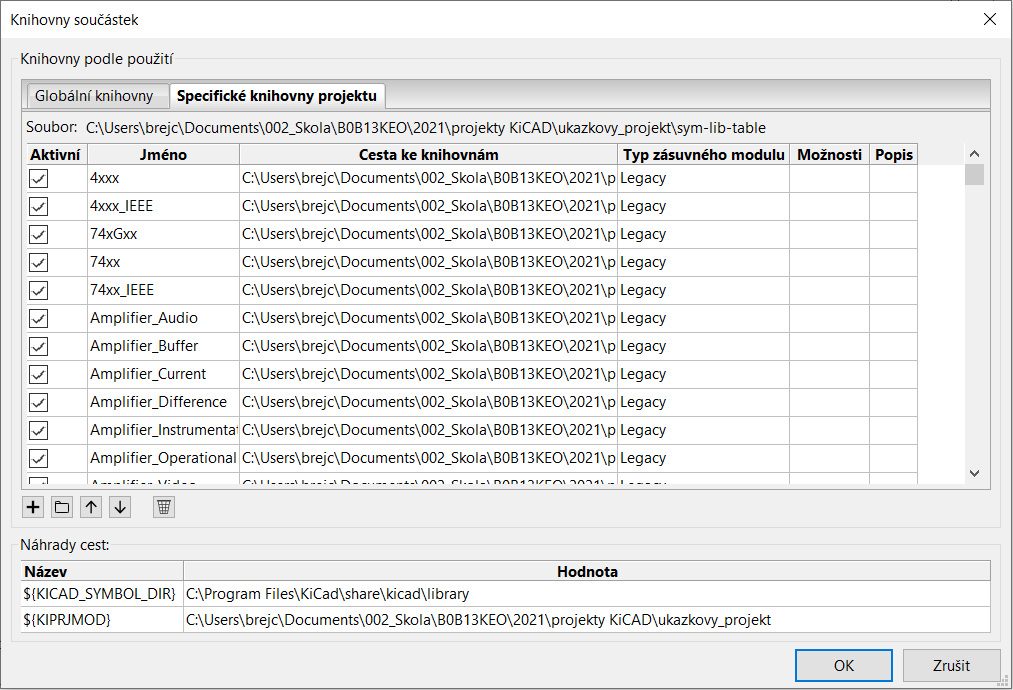
\includegraphics[width=0.85\textwidth]{obr/knihovny05.png}
		\end{center}
		
\end{frame}
%------------------------------------------------------------------------------
\begin{frame}
	\frametitle{Zadání cest ke knihovnám - schematické značky}

		\begin{center}
			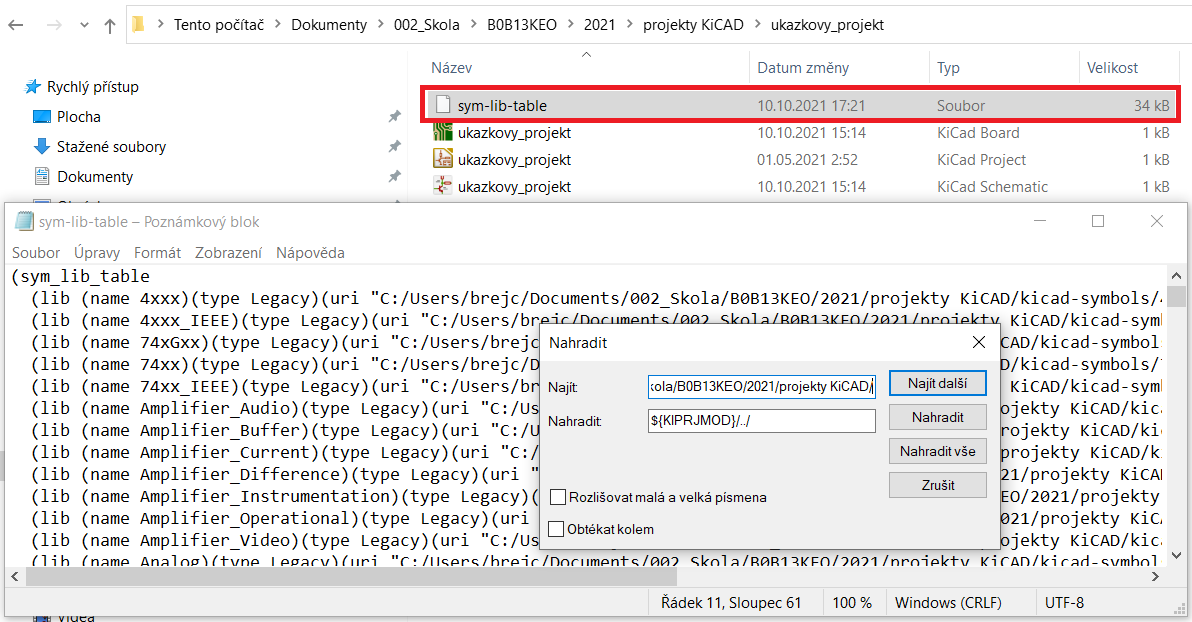
\includegraphics[width=0.85\textwidth]{obr/knihovny06.png}
		\end{center}
		
		Praktickou cestou je otevření projektového souboru sym-lib-table v poznámkovém bloku a provedení hromadného nahrazení textu.
\end{frame}
%------------------------------------------------------------------------------
\begin{frame}
	\frametitle{Zadání cest ke knihovnám - schematické značky}

		\begin{center}
			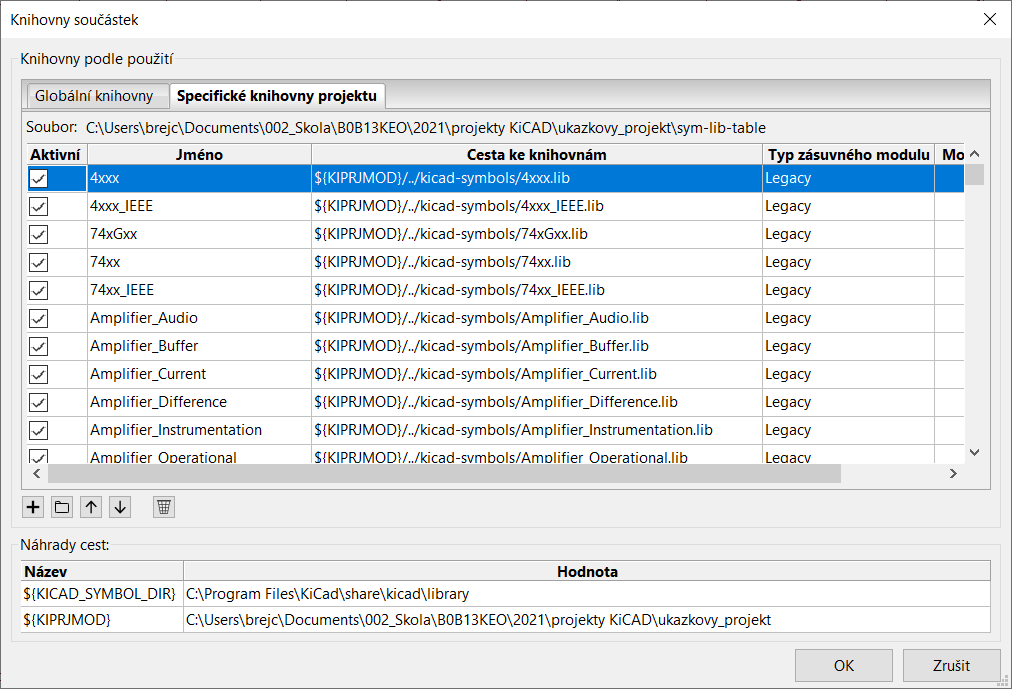
\includegraphics[width=0.85\textwidth]{obr/knihovny07.png}
		\end{center}
		
\end{frame}
%------------------------------------------------------------------------------
\begin{frame}
	\frametitle{Zadání cest ke knihovnám - pouzdra}
		
		Téměř identický postup je třeba udělat ještě pro knihovny pouzder. Zde zadáváme cesty k adresářům s koncovkou *.pretty
		
		\vspace{3mm}
		Při zadávání dejte pozor, ať \textbf{nepřidáváte tyto adresáře}:
		
		\begin{itemize}
		  \item .github
			\item CMakeModules,
		  \item Obsolete,
			\item Sources.
		\end{itemize}
		
		Tyto adresáře jsou vždy součástí stažených knihoven a nejedná se o knihovní prvky.
		
		\vspace{3mm}
		Změnu absolutních cest na relativní proveďte ve vytvořeném souboru fp-lib-table.
\end{frame}
%------------------------------------------------------------------------------
\begin{frame}
	\frametitle{Zadání cest ke knihovnám - pouzdra}

		\begin{center}
			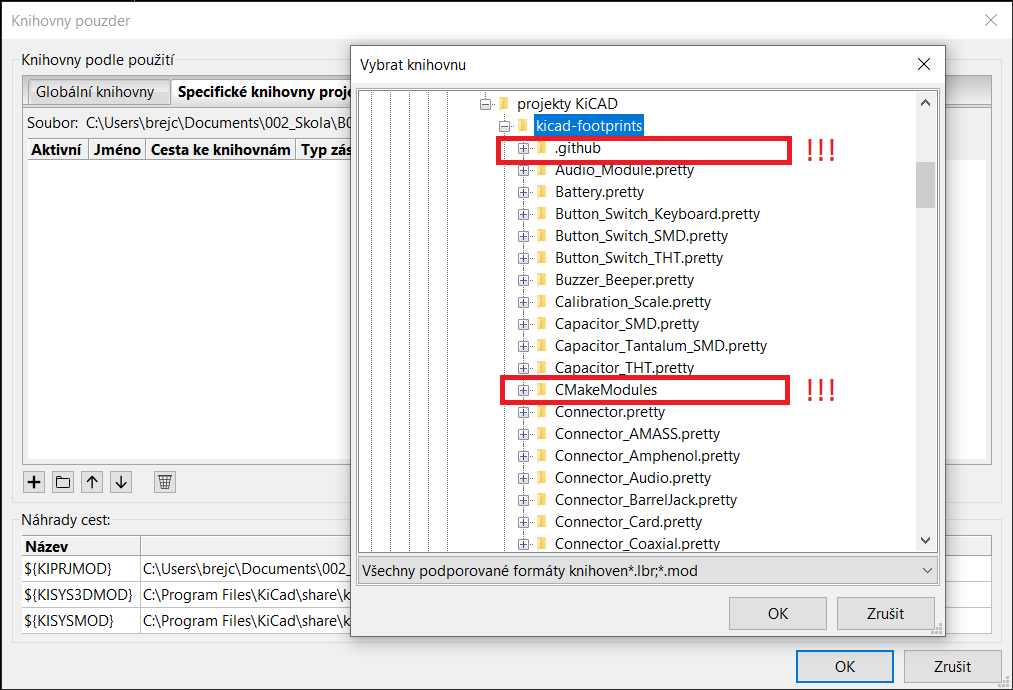
\includegraphics[width=0.85\textwidth]{obr/knihovny08.png}
		\end{center}
		
\end{frame}
%------------------------------------------------------------------------------

%------------------------------------------------------------------------------
% Eeschema
%------------------------------------------------------------------------------
\section{\texorpdfstring{Schéma zapojení}{Schema zapojeni}}
%------------------------------------------------------------------------------
\begin{frame}
	\frametitle{Spuštění Eeschema}

		\begin{center}
			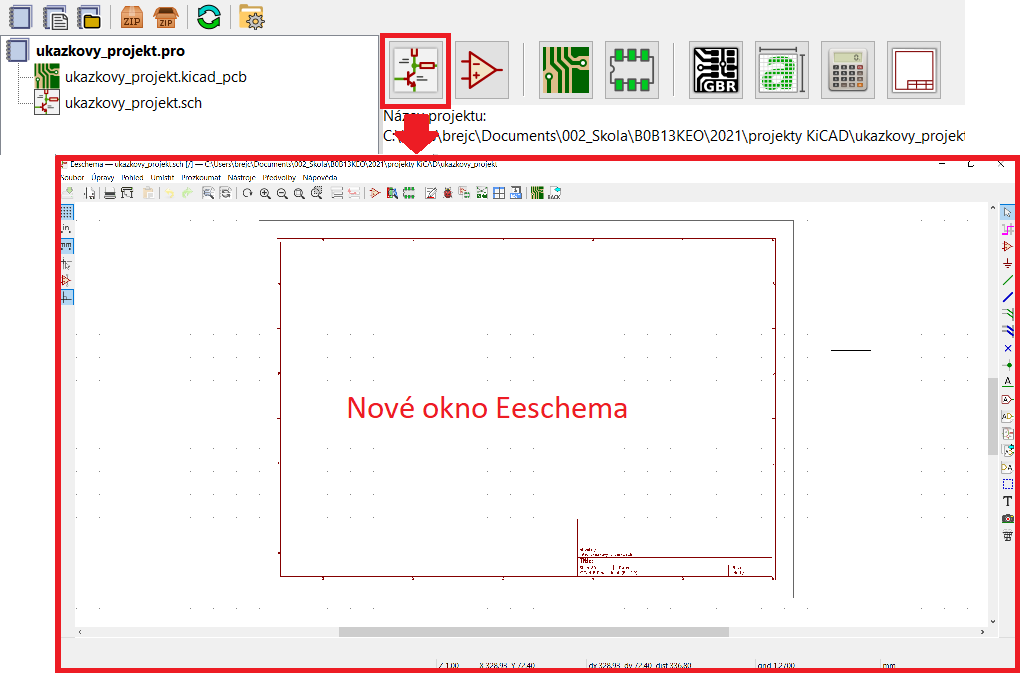
\includegraphics[width=0.9\textwidth]{obr/Eeschema.png}
		\end{center}
		
\end{frame}
%------------------------------------------------------------------------------
\begin{frame}
	\frametitle{Základní ovládání}
	
	\begin{itemize}
		\item \textbf{Levé tlačítko myši:}
		
		\begin{itemize}
			\item Výběr prvků,
			\item tažením lze vybrat více prvků najednou,
			\item dvojím kliknutím lze vyvolat volbu nastavení konkrétní položky.
		\end{itemize}
		
		\item \textbf{Pravé tlačítko myši:}
		
		\begin{itemize}
			\item U konkrétních prvků nabízí místní nabídku možností úprav prvku.
		\end{itemize}
		
		\item \textbf{Kolečko myši:}
		
		\begin{itemize}
			\item Točení přibližuje a oddaluje,
			\item stisk drží stránku a je tak možné se přemisťovat po stránce tažením myši.
		\end{itemize}
		
	\end{itemize}
		
\end{frame}
%------------------------------------------------------------------------------

%------------------------------------------------------------------------------
\subsection{\texorpdfstring{Volba stránky a razítko}{Volba stranky a razitko}}
%------------------------------------------------------------------------------
\begin{frame}
	\frametitle{Volba stránky a razítko}
	\begin{columns}
	
		\column{0.5\textwidth}
		\small
		\begin{itemize}
			\item Ikona stranky vlevo nahore
			\item $\downarrow$ Soubor $\downarrow$ Nastavení stránky
		\end{itemize}
		
		\column{0.5\textwidth}
		\begin{center}
			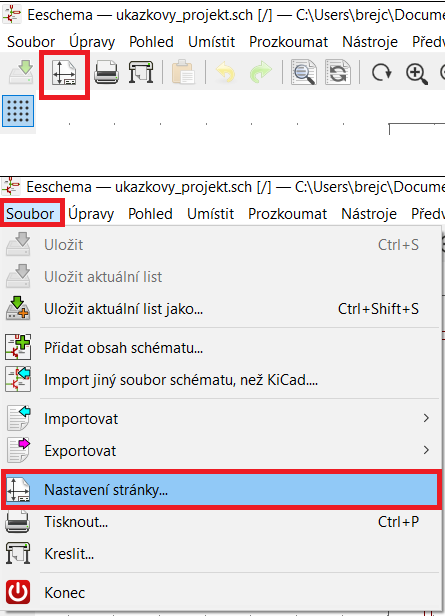
\includegraphics[width=0.8\textwidth]{obr/razitko01.png}
		\end{center}
		
	\end{columns}
\end{frame}
%------------------------------------------------------------------------------
\begin{frame}
	\frametitle{Volba stránky a razítko}
	\begin{columns}
	
		\column{0.3\textwidth}
		\small
		\textcolor{red}{Vlevo}
		\begin{itemize}
			\item nastavení stránky
		\end{itemize}
		\textcolor{blue}{Vpravo}
		\begin{itemize}
			\item vyplnění razítka
		\end{itemize}
		
		\column{0.7\textwidth}
		\begin{center}
			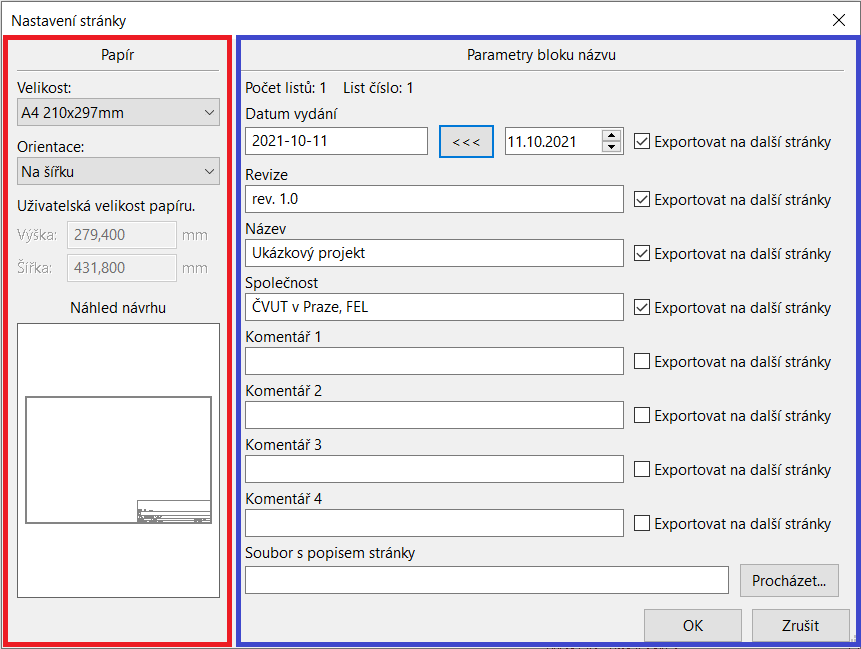
\includegraphics[width=\textwidth]{obr/razitko02.png}
		\end{center}
		
	\end{columns}
	
	
	\begin{itemize}
		\item Údaje na razítku je možné přenést na všechny stránky projektu po zaškrtnutí \uv{Exportovat na další stránky}.
	\end{itemize}
\end{frame}
%------------------------------------------------------------------------------
\begin{frame}
	\frametitle{Volba stránky a razítko}

		\begin{center}
			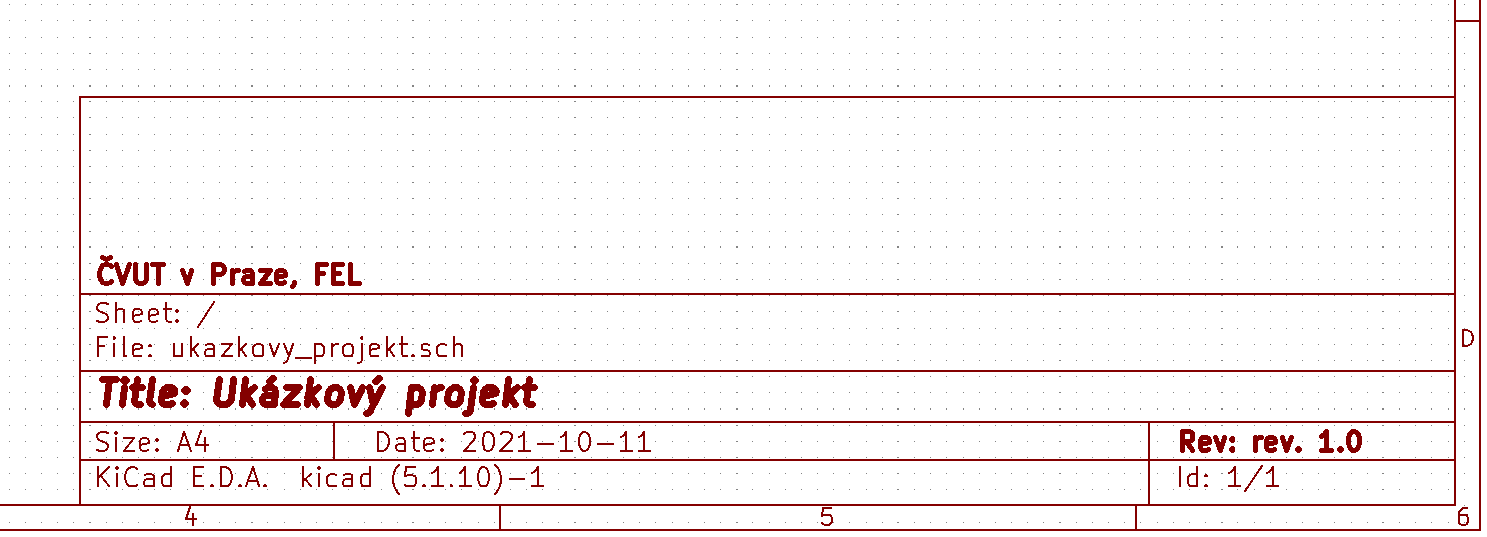
\includegraphics[width=0.9\textwidth]{obr/razitko03.png}
		\end{center}
		
		Nastavení stránky a vyplnění razítka lze zkontrolovat v levém spodním okraji stránky Eeschema.
\end{frame}
%------------------------------------------------------------------------------


%------------------------------------------------------------------------------
\subsection{\texorpdfstring{Vkládání součástek}{Vkladani soucastek}}
%------------------------------------------------------------------------------
\begin{frame}
	\frametitle{Výběr a vložení součástky}
	\begin{columns}
	
		\column{0.45\textwidth}
		\small
		\begin{enumerate}
			\item $\downarrow$ Umístit $\downarrow$ Součástka,
			\item svislé menu vpravo, ikona OZ,
			\item \uv{SHIFT + A} nebo jen \uv{A}
		\end{enumerate}
		
		\column{0.55\textwidth}
		\begin{center}
			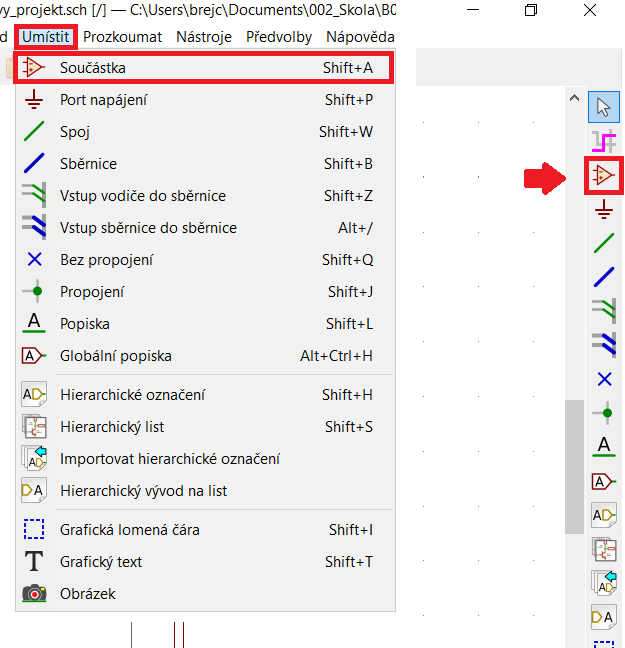
\includegraphics[width=\textwidth]{obr/umisti_soucastku01.png}
		\end{center}
		
	\end{columns}
\end{frame}
%------------------------------------------------------------------------------
\begin{frame}
	\frametitle{Výběr a vložení součástky}
	\begin{columns}
	
		\column{0.55\textwidth}
		\small
		\begin{enumerate}
			\item Filtr pro vyhledávání symbolů,
			\item nabídka všech nebo filtrovaných symbolů,
			\item náhled vybraného symbolu,
			\item popis vybraného symbolu.
		\end{enumerate}
		
		\textbf{Filtrování}
		\begin{itemize}
			\item buď zadáním počátku názvu symbolu,
			\item nebo lze s jistými omezeními zadat regulární výraz.
		\end{itemize}
		
		\textbf{Zkuste zadat:} 74HC, 74HC7, 74??74, 74*74, 74\textbackslash w+74 apod.
		
		\column{0.45\textwidth}
		\begin{center}
			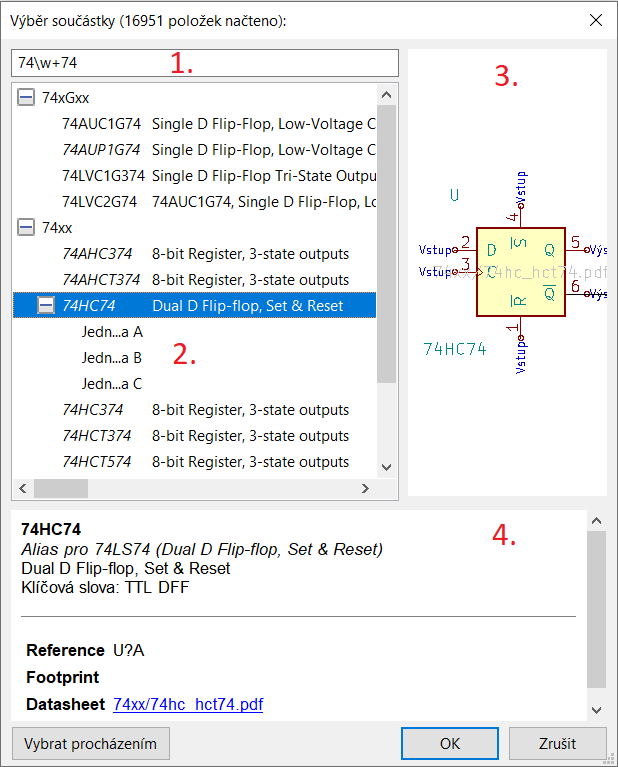
\includegraphics[width=\textwidth]{obr/umisti_soucastku02.png}
		\end{center}
		
	\end{columns}
\end{frame}
%------------------------------------------------------------------------------
\begin{frame}
	\frametitle{Výběr a vložení součástky}
	
	\begin{itemize}
		\item Po stisku \uv{OK} se symbol vybere a je jím možné volně pohybovat po pracovní ploše,
		\item kliknutím levým tlačítkem myši symbol umístíme.
	\end{itemize}
	
	\textbf{Úpravy:}
	
	Pravým kliknutím myši na symbol se  zobrazí nabídka úprav, z nichž nejdůležitější jsou tyto:
	
	\begin{center}
		\begin{tabular}{| c | l |}
			\hline
			\textbf{Klávesa} & \textbf{Popis} \\ \hline
			M & Přesun symbolu \\ \hline
			\textcolor{blue}{\textbf{V}} & \textcolor{blue}{\textbf{Změna hodnoty součástky}} \\ \hline
			R & Rotace, otočení symbolu \\ \hline
			X & Zrcadlení podle horizontální osy \\ \hline
			Y & Zrcadlení podle vertikální osy \\ \hline
			E & Úprava parametrů symbolu \\ \hline
			C & Kopírování, klonování, duplikování symbolu \\ \hline
		\end{tabular}
	\end{center}
	
\end{frame}
%------------------------------------------------------------------------------
\begin{frame}
	\frametitle{Hodnota součástky}
	
	\begin{itemize}
		\item Hodnotu lze zapsat (změnit) po najetí myši nad součástku a stisku klávesy \uv{V} nebo dvojím kliknutím na danou hodnotu.
		\item Hodnoty zapisujme ve tvaru, kde desetinnou čárku nahrazujeme písmenem označující řády.
	\end{itemize}
	
	\hrule
	
	\begin{itemize}
		\item Typické značení řádů u rezistorů:
		
		\begin{itemize}
			\item R = $10^0$: $0,47$ $\Omega$ je ve schéma 0R47, $10$ $\Omega$ je je ve schéma 10R,
			\item k = $10^3$: $1200$ $\Omega$ je ve schéma 1k2, $10000$ $\Omega$ je je ve schéma 10k,
			\item M = $10^6$: $1,2$ M$\Omega$ je ve schéma 1M2 atd.
		\end{itemize}
		
		\item Typické značení řádů u kondenzátorů:
		
		\begin{itemize}
			\item p = $10^{-12}$: $220$ pF je ve schéma 220p,
			\item n = $10^{-9}$: $1,2$ nF je ve schéma 1n2, $220$ nF je ve schéma 220n,
			\item u = $10^{-6}$: $1,2$ $\mu$F je ve schéma 1u2, $47$ $\mu$F je ve schéma 47u,
			\item m = $10^{-3}$: $1,2$ mF je ve schéma 1m2,
		\end{itemize}
	\end{itemize}
	
\end{frame}
%------------------------------------------------------------------------------
\begin{frame}
	\frametitle{Víceprvkové symboly}
	\small
	\begin{itemize}
		\item Některé symboly se skládají z několika prvků.
		\item V knihovně je to vidět tak, že po rozbalení jména prvku (+) se objeví další symboly pojmenované jako \uv{jednotka A}, \uv{jednotka B} atd.
		\item Typickými zástupci jsou logické obvody jako je například D klopný obvod 74HC74. Každá jednotka zastupuje jedno hradlo nebo napájecí vstupy.
	\end{itemize}
	
	\begin{center}
		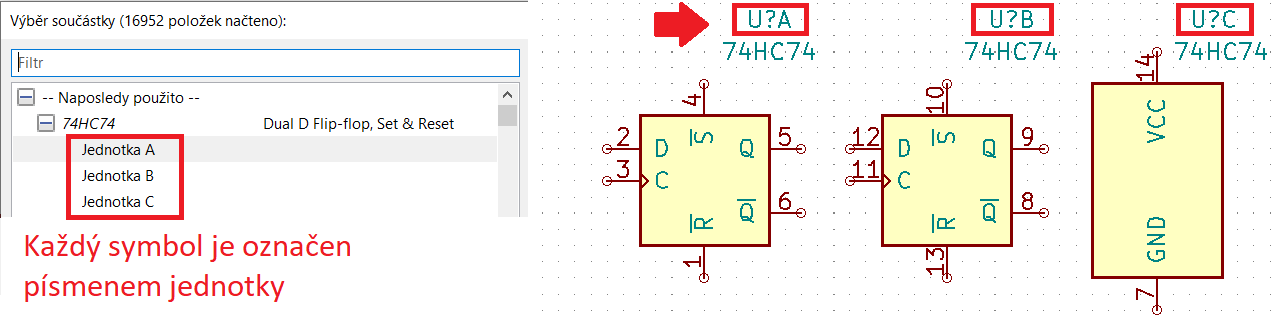
\includegraphics[width=\textwidth]{obr/umisti_soucastku03.png}
	\end{center}
	
\end{frame}
%------------------------------------------------------------------------------
\begin{frame}
	\frametitle{Víceprvkové symboly}
	\small
	\begin{itemize}
		\item \textbf{Do schéma zapojení bychom měli vždy vkládat všechny jednotky daného symbolu.}
		\item Pokud klonujeme resp. kopírujeme víceprvkový symbol, pak se vždy zkopíruje aktuální jednotka.
		\item Jednotku daného prvku lze změnit úpravou vlastností (pravé tlačítko myši na symbolu: $\downarrow$ Vlastnosti $\downarrow$ upravit vlastnosti, nebo klávesa \uv{e})
	\end{itemize}
	
	\begin{center}
		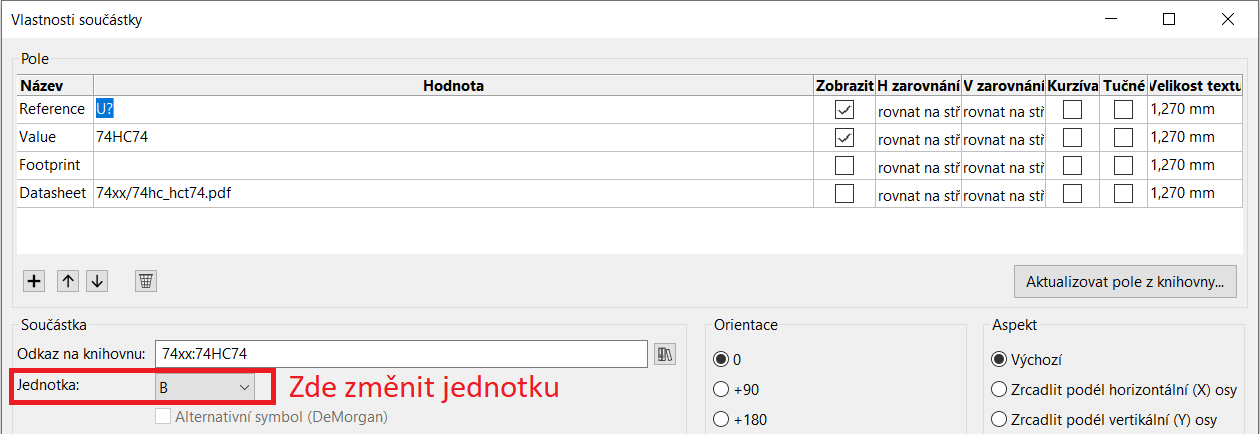
\includegraphics[width=\textwidth]{obr/umisti_soucastku04.png}
	\end{center}
	
\end{frame}
%------------------------------------------------------------------------------


%------------------------------------------------------------------------------
\subsection{\texorpdfstring{Propojování - vodiče a odkazy}{Propojovani - vodice a odkazy}}
%------------------------------------------------------------------------------
\begin{frame}
	\frametitle{Propojování vodiči}
	\begin{columns}
	
		\column{0.45\textwidth}
		\small
		\begin{enumerate}
			\item $\downarrow$ Umístit $\downarrow$ Spoj,
			\item svislé menu vpravo, ikona zelené čáry,
			\item \uv{SHIFT + W} nebo jen \uv{W}
		\end{enumerate}
		
		\column{0.55\textwidth}
		\begin{center}
			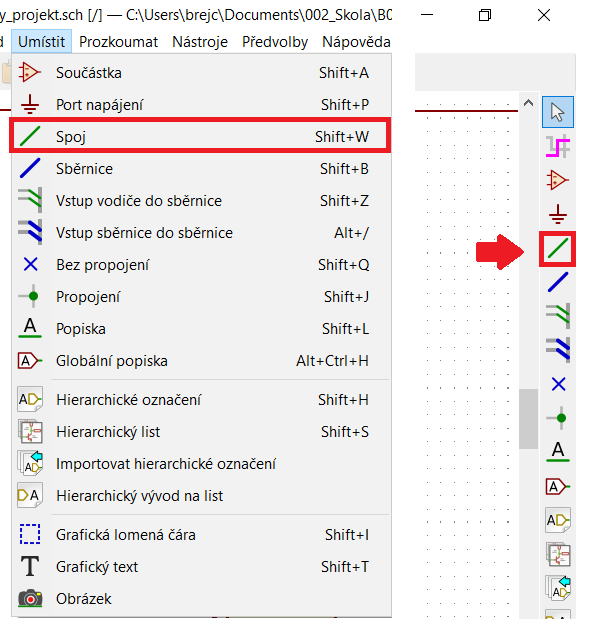
\includegraphics[width=\textwidth]{obr/spoje01.png}
		\end{center}
		
	\end{columns}
\end{frame}
%------------------------------------------------------------------------------
\begin{frame}
	\frametitle{Propojování vodiči}
	
	\begin{center}
		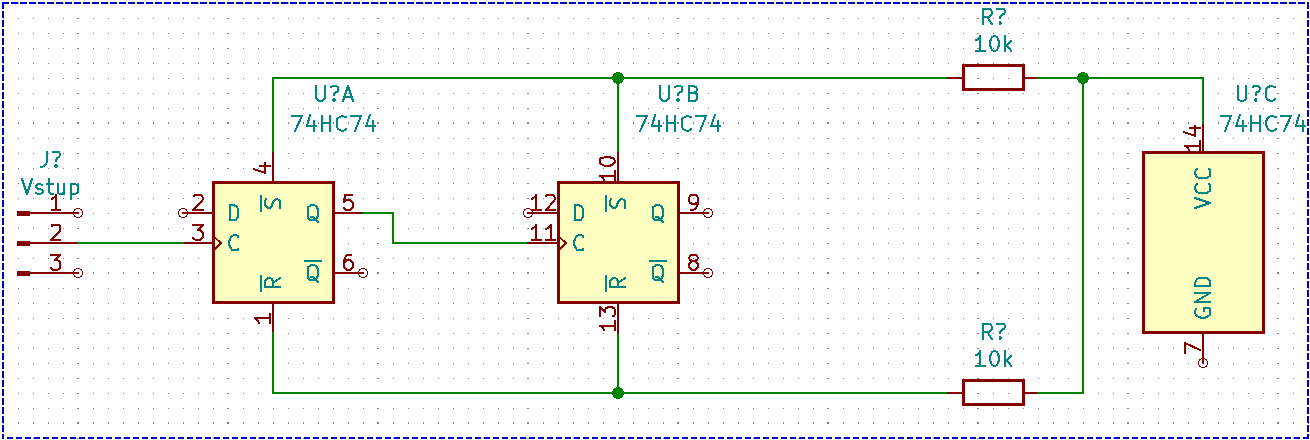
\includegraphics[width=\textwidth]{obr/spoje02.png}
	\end{center}
	
	\small
	
	\begin{itemize}
		\item Kliknutím levým tlačítkem zahájíme spoj,
		\item kliknutím mimo vývod součástky vytváříme ohyb (koleno) ve spoji,
		\item kliknutím na vývod součástky nebo jiný vodič se aktivní vodič připojí a ukončí.
		\item Uzly se vytvářejí sami, pokud vodič končí na jiném vodiči, nebo je lze přidávat z menu vpravo, ikona zeleného puntíku.
	\end{itemize}
	
\end{frame}
%------------------------------------------------------------------------------
\begin{frame}
	\frametitle{Propojování globálními popisky}
	\begin{columns}
	
		\column{0.45\textwidth}
		\small
		\begin{enumerate}
			\item Globální popisky se symbolem,
			\item vlastní globální popisky.
		\end{enumerate}
		
		Ad 1.:
		\begin{itemize}
			\item Přidávat jako součástku (GND, +5V, ...),
			\item nebo jako symbol napájení \uv{SHIFT + P} nebo jen \uv{P}
		\end{itemize}
		
		Ad 2.:
		\begin{itemize}
			\item $\downarrow$ Umístit $\downarrow$ Globální popiska,
			\item svislé menu vpravo, ikona \uv{A} v praporku.
		\end{itemize}
		
		\column{0.55\textwidth}
		\begin{center}
			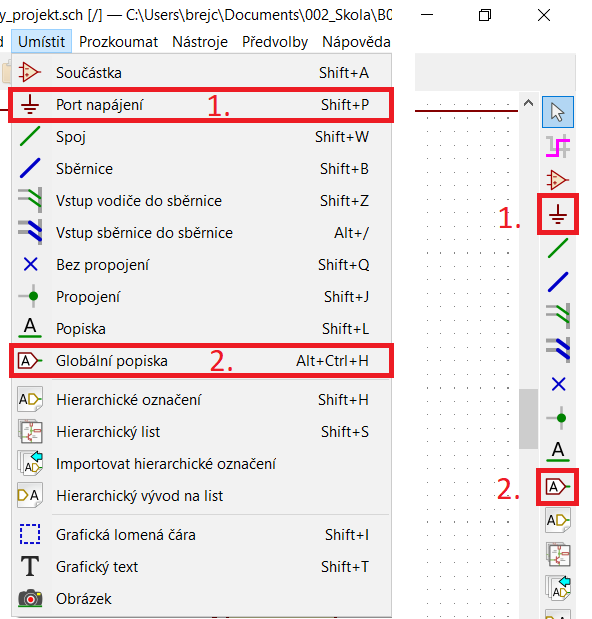
\includegraphics[width=\textwidth]{obr/spoje03.png}
		\end{center}
		
	\end{columns}
\end{frame}
%------------------------------------------------------------------------------
\begin{frame}
	\frametitle{Propojování globálními popisky}
	
	\begin{center}
		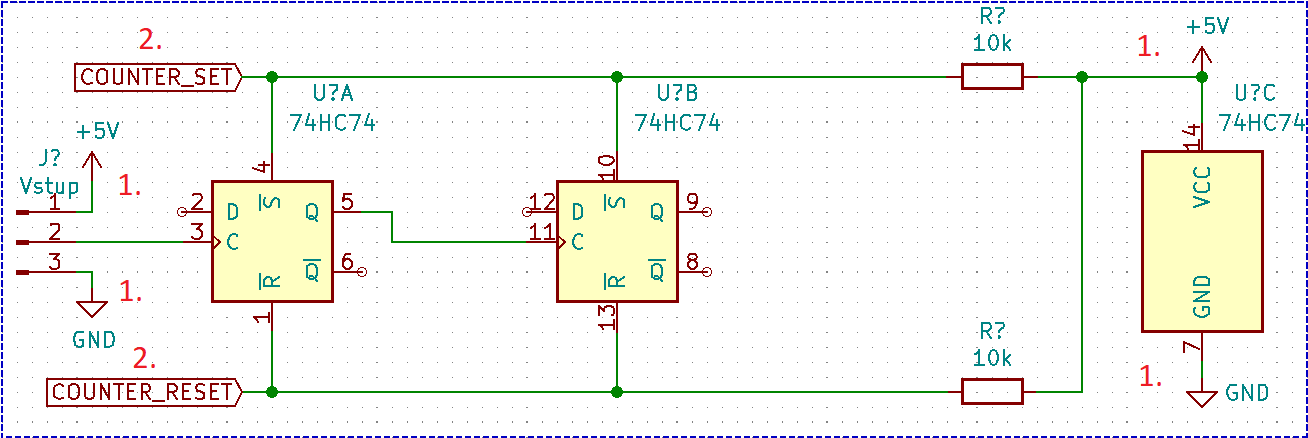
\includegraphics[width=\textwidth]{obr/spoje04.png}
	\end{center}
	
	\small
	
	\begin{itemize}
		\item Globální popisky jsou viditelné ze všech listů, proto je kvůli přehlednosti používejte obezřetně.
		\item U napájení je vhodné použít přímo symboly s napěťovou reprezentací.
	\end{itemize}
	
\end{frame}
%------------------------------------------------------------------------------
\begin{frame}
	\frametitle{Propojování lokálními popisky}
	\begin{columns}
	
		\column{0.45\textwidth}
		\small
		\begin{enumerate}
			\item $\downarrow$ Umístit $\downarrow$ Popiska,
			\item svislé menu vpravo, ikona zeleně pod škrtnutého písmena A,
			\item \uv{SHIFT + L} nebo jen \uv{L}
		\end{enumerate}
		
		\column{0.55\textwidth}
		\begin{center}
			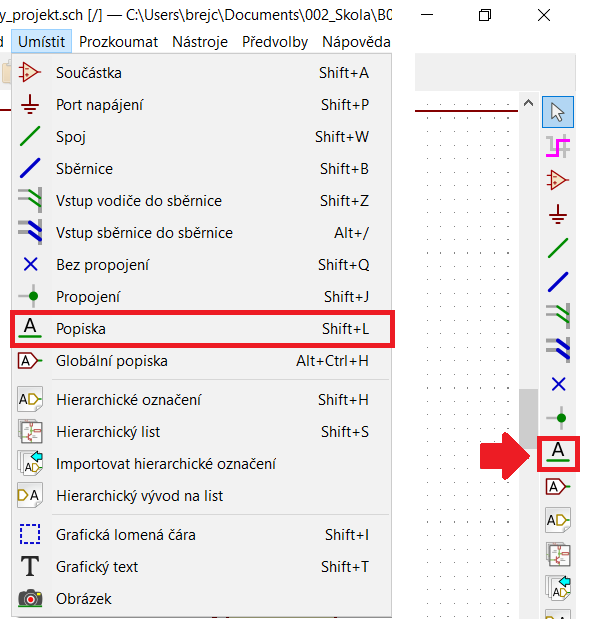
\includegraphics[width=\textwidth]{obr/spoje05.png}
		\end{center}
		
	\end{columns}
\end{frame}
%------------------------------------------------------------------------------
\begin{frame}
	\frametitle{Propojování lokálními popisky}
	
	\begin{center}
		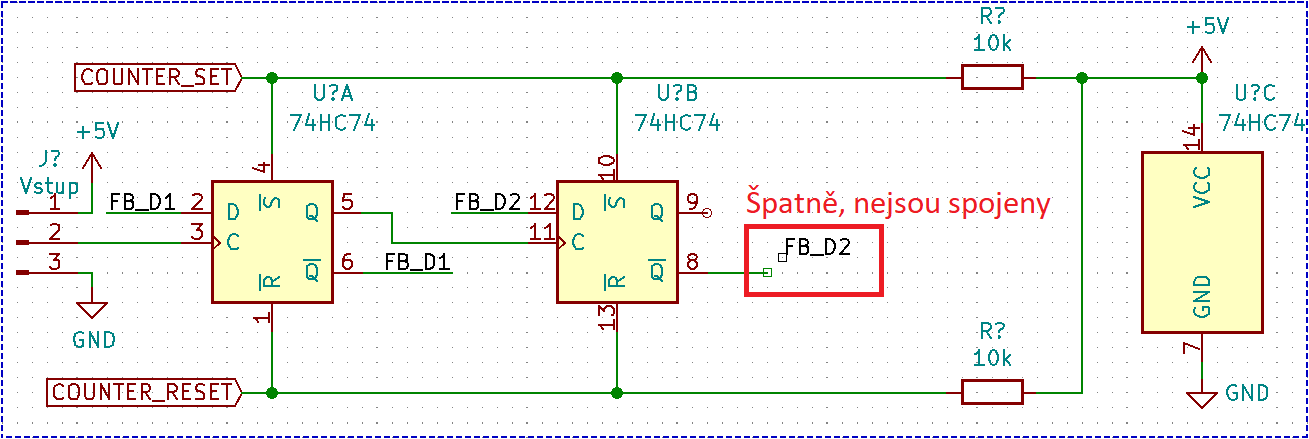
\includegraphics[width=\textwidth]{obr/spoje06.png}
	\end{center}
	
	\small
	
	\begin{itemize}
		\item Do zobrazeného pole zapište název popisku. Popisek lze opakovaně editovat dvojím kliknutím nebo stiskem klávesy \uv{E}.
		\item Popisky jsou platné jen v rámci daného listu.
		\item Popisek lze umístit na ukončený i neukončený vodič. Neukončený vodič lze vytvořit při jeho kreslení dvojím kliknutím.
	\end{itemize}
	
\end{frame}
%------------------------------------------------------------------------------


%------------------------------------------------------------------------------
\subsection{\texorpdfstring{Tvorba nových listů}{Tvorba novych listu}}
%------------------------------------------------------------------------------
\begin{frame}
	\frametitle{Přidávání listů}
	\begin{columns}
	
		\column{0.45\textwidth}
		\small
		\begin{enumerate}
			\item $\downarrow$ Umístit $\downarrow$ Hierarchický list,
			\item svislé menu vpravo, ikona schéma,
			\item \uv{SHIFT + S} nebo jen \uv{S}
		\end{enumerate}
		
		\column{0.55\textwidth}
		\begin{center}
			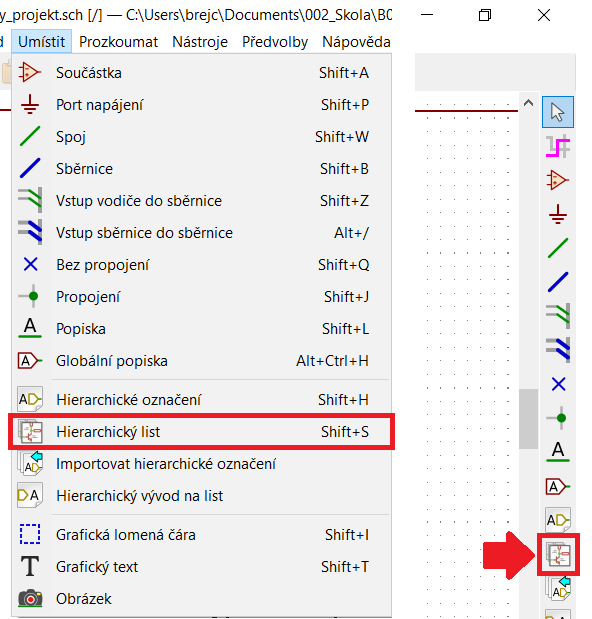
\includegraphics[width=\textwidth]{obr/dalsi_strana01.png}
		\end{center}
		
	\end{columns}
\end{frame}
%------------------------------------------------------------------------------
\begin{frame}
	\frametitle{Přidávání listů}
	
	\begin{center}
		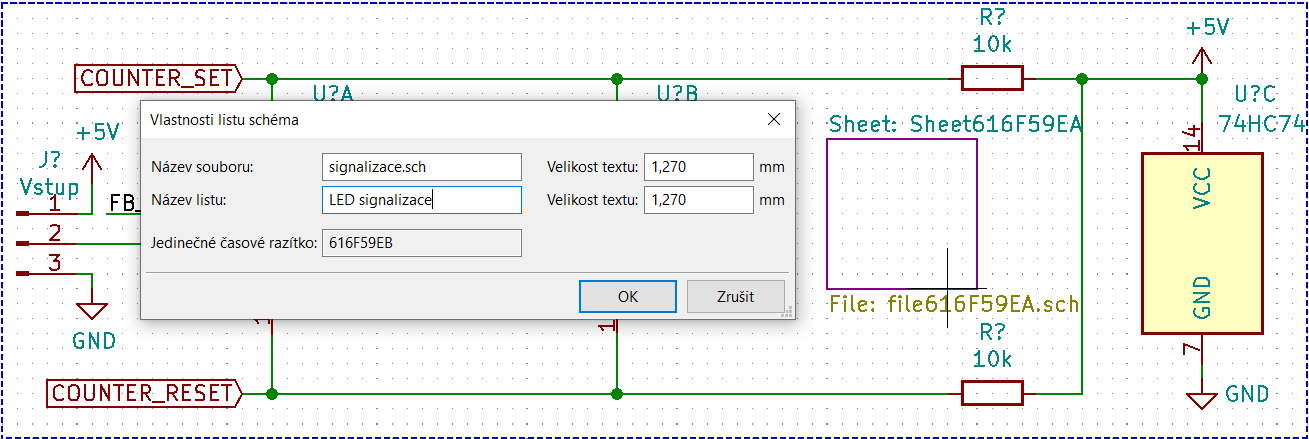
\includegraphics[width=\textwidth]{obr/dalsi_strana02.png}
	\end{center}
	
	\small
	
	\begin{itemize}
		\item Kliknutím, tažením a dalším kliknutím vytvořte blok ve schématu.
		\item Zapište jméno souboru a název listu.
	\end{itemize}
	
\end{frame}
%------------------------------------------------------------------------------
\begin{frame}
	\frametitle{Přidávání listů}
	
	\begin{itemize}
		\item Do nového listu se dostanete dvojím kliknutím na vytvořený blok.
		\item Do kteréhokoliv místa v projektu se můžete dostat pomocí navigátoru:
			\begin{center}
				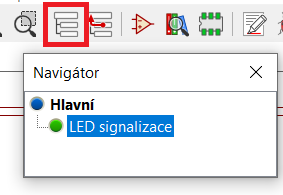
\includegraphics[scale=0.6]{obr/dalsi_strana03.png}
			\end{center}
		\item Do listu o úroveň výš se dostanete ikonou s červenou šipkou:
			\begin{center}
				
\includegraphics[scale=0.6]{obr/dalsi_strana04.png}
			\end{center}
	\end{itemize}
	
\end{frame}
%------------------------------------------------------------------------------
\begin{frame}
	\frametitle{Propojení mezi listy}
	\begin{columns}
	
		\column{0.45\textwidth}
		\small
		
		\begin{itemize}
			\item Ve všech listech platí globální popisky,
			\item signály mezi listy lze vést pomocí vývodů.
		\end{itemize}
		
		\textbf{Přidání vývodu:}
		\begin{enumerate}
			\item $\downarrow$ Umístit $\downarrow$ Hierarchické označení,
			\item svislé menu vpravo, ikona písmene A mimo praporek,
			\item \uv{SHIFT + H} nebo jen \uv{H}
		\end{enumerate}
		
		\column{0.55\textwidth}
		\begin{center}
			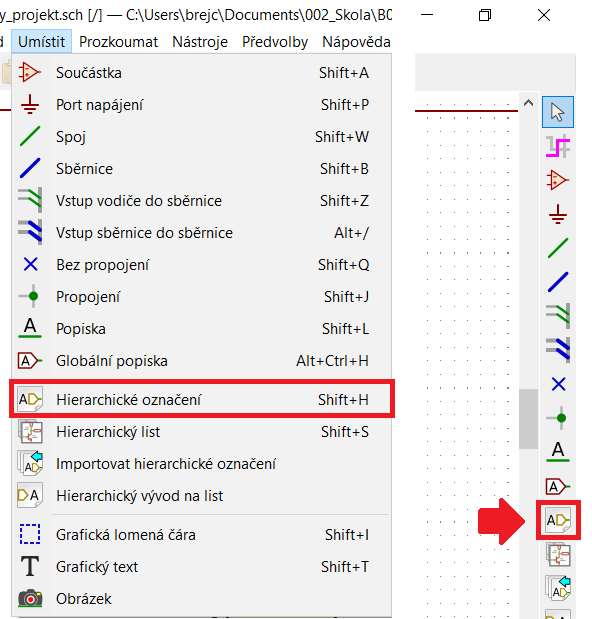
\includegraphics[width=\textwidth]{obr/dalsi_strana05.png}
		\end{center}
		
	\end{columns}
\end{frame}
%------------------------------------------------------------------------------
\begin{frame}
	\frametitle{Propojení mezi listy}
	\small
	Definice vývodu:
	
	\begin{itemize}
		\item Název,
		\item orientaci není třeba nastavovat, s vývodem lze rotovat,
		\item styl se týká zobrazení,
		\item vždy nastavujte příslušný tvar, který určuje zda se jedná o vstup, výstup atd.
	\end{itemize}
	
	\begin{center}
		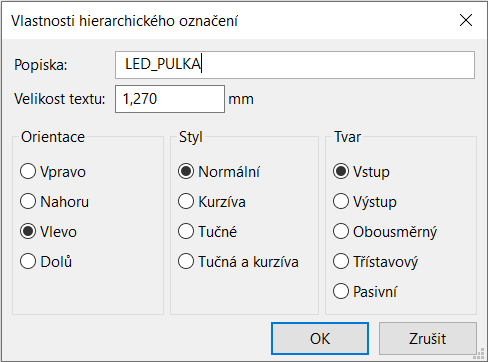
\includegraphics[scale=0.5]{obr/dalsi_strana06.png}
	\end{center}

\end{frame}
%------------------------------------------------------------------------------
\begin{frame}
	\frametitle{Propojení mezi listy}
	\small
	\begin{itemize}
		\item Obvyklou praxí je umisťování vstupů vlevo a výstupů vpravo jak pro schéma zapojení tak pro list.
			\begin{center}
				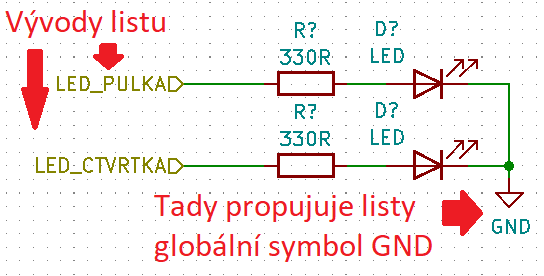
\includegraphics[width=0.4\textwidth]{obr/dalsi_strana07.png}
			\end{center}
		\item Volba tvaru (typu) propojení mezi listy je přehledná pro každého, kdo zdědí a chce pokračovat ve vašem projektu.
			\begin{center}
				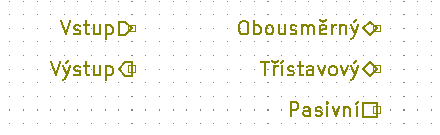
\includegraphics[width=0.4\textwidth]{obr/dalsi_strana08.png}
			\end{center}
		\item Propojování vývody je vhodnější než propojování globálními popisky, protože zachovává návaznost listů.
	\end{itemize}
	
\end{frame}
%------------------------------------------------------------------------------



%------------------------------------------------------------------------------
\subsection{\texorpdfstring{Kontrola zapojení}{Kontrola zapojeni}}
%------------------------------------------------------------------------------
\begin{frame}
	\frametitle{Kontrola zapojení}
		
\end{frame}
%------------------------------------------------------------------------------


%-----------------------------------------------------------------------------
\subsection{\texorpdfstring{Přiřazení pouzder}{Prirazeni pouzder}}
%------------------------------------------------------------------------------
\begin{frame}
	\frametitle{Přiřazování pouzder}
		
\end{frame}
%------------------------------------------------------------------------------

  
\end{document}